\documentclass[11pt,letterpaper]{article}

% ---------------------------------------------------------
% Paquetes
% ---------------------------------------------------------
\usepackage[utf8]{inputenc}
\usepackage[T1]{fontenc}
\usepackage[spanish]{babel}
\usepackage{graphicx}
\usepackage{geometry}
\usepackage{amsmath}
\usepackage{listings}
\usepackage{xcolor}
\usepackage{float}
\usepackage[hidelinks]{hyperref}

\geometry{letterpaper, margin=2.1cm}

% ---------------------------------------------------------
% Configuración de código
% ---------------------------------------------------------
\lstset{
    language=Python,
    basicstyle=\ttfamily\footnotesize,
    keywordstyle=\color{blue},
    commentstyle=\color{gray},
    stringstyle=\color{red!60!black},
    numbers=left,
    numberstyle=\tiny,
    frame=single,
    breaklines=true,
    showstringspaces=false,
    columns=fullflexible
}

% ---------------------------------------------------------
% Datos
% ---------------------------------------------------------
\title{Taller 4: Vecindad, Ecualización Local y Operaciones Lógicas}
\author{
Camilo Eduardo Muñoz Albornoz\\
Procesamiento Digital de Imágenes\\
Universidad Tecnológica de Pereira
}
\date{}

\begin{document}

\maketitle

% =========================================================
\begin{abstract}
En este taller se estudiaron conceptos de vecindad de píxeles, procesamiento local de imágenes y operaciones lógicas binarias. Se implementaron funciones para obtener los ocho vecinos de un píxel, se analizaron distintas posiciones dentro de una imagen, se aplicó ecualización local mediante estadísticas de vecindad y se implementaron operaciones AND, OR, XOR y NOT entre imágenes binarias. Los algoritmos fueron desarrollados en Python utilizando OpenCV y NumPy.
\end{abstract}


% =========================================================
\section{Objetivos}

Los objetivos del taller fueron:

\begin{enumerate}
    \item Crear una función que determine las intensidades de los ocho vecinos de un píxel definido por coordenadas suministradas por el usuario.
    
    \item Probar el algoritmo de vecindad con una imagen en escala de grises.
    
    \item Aplicar la función sobre la imagen \texttt{PIANO.bmp} en las coordenadas:
    \[
    (82,29),\ (68,27),\ (112,89),\ (114,89),\ (27,130)
    \]
    
    \item Ejecutar una ecualización local sobre una imagen y comparar la imagen original, la transformada y sus respectivos histogramas.
    
    \item Implementar manualmente mediante ciclos la ecualización local utilizando la imagen \texttt{PIANO.pgm}, limitando el factor de realce al intervalo:
    \[
    0.5 \leq A(i,j) \leq 2.5
    \]
    
    \item Crear funciones basadas en ciclos para realizar las operaciones lógicas AND, OR, XOR y NOT entre imágenes binarias y verificar su funcionamiento con \texttt{CuadroBinGrande.pgm} y \texttt{CuadroBinChico.pgm}.
\end{enumerate}


% =========================================================
\section{Fundamentos teóricos}

\subsection{Vecindad de un píxel}

En una imagen digital, un píxel no solamente puede analizarse de manera individual. También puede estudiarse teniendo en cuenta los píxeles que lo rodean.

Para un píxel $p(x,y)$ se pueden definir diferentes tipos de vecindad.

La vecindad de cuatro píxeles considera las posiciones:

\[
N_4(p)=
\{
(x-1,y),
(x+1,y),
(x,y-1),
(x,y+1)
\}
\]

La vecindad diagonal considera:

\[
N_D(p)=
\{
(x-1,y-1),
(x+1,y-1),
(x-1,y+1),
(x+1,y+1)
\}
\]

La vecindad de ocho píxeles corresponde a la unión de ambas:

\[
N_8(p)=N_4(p)\cup N_D(p)
\]

Por tanto, alrededor de un píxel central se obtiene una estructura:

\[
\begin{bmatrix}
p_1 & p_2 & p_3\\
p_4 & p   & p_5\\
p_6 & p_7 & p_8
\end{bmatrix}
\]

En NumPy y OpenCV una imagen se accede mediante:

\[
\texttt{imagen[y,x]}
\]

es decir, primero la fila y después la columna.

Este concepto es importante porque muchas técnicas de procesamiento de imágenes dependen de la información local, por ejemplo filtrado, detección de bordes, segmentación y análisis de textura.


% =========================================================
\subsection{Media y desviación estándar local}

Para analizar una región alrededor de un píxel puede utilizarse una ventana, por ejemplo de:

\[
3\times3
\]

que incluye el píxel central y sus ocho vecinos.

La media local se define como:

\[
\bar{x}(i,j)=
\frac{1}{N}
\sum_{n=1}^{N}x_n
\]

donde $N$ representa el número de píxeles de la ventana.

Para una ventana $3\times3$:

\[
N=9
\]

La desviación estándar local permite medir qué tan diferentes son las intensidades dentro de esa región:

\[
\sigma(i,j)
=
\sqrt{
\frac{1}{N}
\sum_{n=1}^{N}
(x_n-\bar{x})^2
}
\]

Una desviación pequeña indica una región relativamente uniforme. Una desviación grande indica que existen diferencias importantes entre los píxeles vecinos.


% =========================================================
\subsection{Ecualización local}

La ecualización local modifica cada píxel teniendo en cuenta las características de su vecindad.

La transformación utilizada fue:

\[
y(i,j)
=
A(i,j)
\left[
x(i,j)-\bar{x}(i,j)
\right]
+
\bar{x}(i,j)
\]

donde:

\begin{itemize}
    \item $x(i,j)$ es el valor original del píxel.
    \item $y(i,j)$ es el valor transformado.
    \item $\bar{x}(i,j)$ es la media local.
    \item $\sigma(i,j)$ es la desviación estándar local.
\end{itemize}

El factor de realce se calcula mediante:

\[
A(i,j)
=
k\frac{\bar{x}_G}{\sigma(i,j)}
\]

donde $\bar{x}_G$ es la media global de la imagen.

Cuando la desviación local es pequeña, el valor de $A$ aumenta y el contraste local puede ser realzado con mayor fuerza. Cuando la desviación local es grande, el factor disminuye y el realce es menor.


% =========================================================
\subsection{Operaciones lógicas}

En una imagen binaria cada píxel puede tomar solamente dos valores:

\[
0 \rightarrow \text{negro}
\]

\[
255 \rightarrow \text{blanco}
\]

Estos valores pueden interpretarse como falso y verdadero respectivamente.

Las principales operaciones utilizadas fueron:

\begin{itemize}
    \item \textbf{AND}: produce blanco solamente cuando ambos píxeles son blancos.
    \item \textbf{OR}: produce blanco cuando al menos uno de los píxeles es blanco.
    \item \textbf{XOR}: produce blanco cuando los dos píxeles son diferentes.
    \item \textbf{NOT}: invierte el valor del píxel.
\end{itemize}


% =========================================================
\section{Desarrollo y resultados}

% =========================================================
\subsection{Punto 1: Función para obtener los ocho vecinos}

Se desarrolló una función que recibe una imagen y las coordenadas $(x,y)$ de un píxel.

La función retorna una matriz de $3\times3$ que conserva la posición espacial de los vecinos. La posición central se representa con $-1$ para indicar que no pertenece al conjunto de vecinos.

El código principal fue:

\begin{lstlisting}
def obtener_8_vecinos(imagen, x, y):
    filas, columnas = imagen.shape[:2]

    if x <= 0 or x >= columnas - 1:
        raise ValueError(
            "La coordenada x esta fuera de los limites."
        )

    if y <= 0 or y >= filas - 1:
        raise ValueError(
            "La coordenada y esta fuera de los limites."
        )

    vecinos = np.array([
        [
            imagen[y-1, x-1],
            imagen[y-1, x],
            imagen[y-1, x+1]
        ],
        [
            imagen[y, x-1],
            -1,
            imagen[y, x+1]
        ],
        [
            imagen[y+1, x-1],
            imagen[y+1, x],
            imagen[y+1, x+1]
        ]
    ], dtype=int)

    return vecinos
\end{lstlisting}

También se desarrolló una segunda versión mediante ciclos:

\begin{lstlisting}
def obtener_8_vecinos_ciclos(imagen, x, y):

    vecinos = np.full((3, 3), -1, dtype=int)

    for dy in range(-1, 2):
        for dx in range(-1, 2):

            if dy == 0 and dx == 0:
                continue

            vecinos[dy+1, dx+1] = (
                imagen[y+dy, x+dx]
            )

    return vecinos
\end{lstlisting}

La implementación con ciclos permite comprender que los vecinos se obtienen mediante desplazamientos relativos de $-1$, $0$ y $+1$ alrededor del píxel central.


% =========================================================
\subsection{Punto 2: Prueba con una imagen}

La función se verificó utilizando una imagen en escala de grises y las coordenadas:

\[
(x,y)=(100,100)
\]

El píxel seleccionado presentó intensidad:

\[
128
\]

y sus ocho vecinos fueron:

\[
\begin{bmatrix}
157 & 124 & 127\\
167 & -1 & 134\\
169 & 126 & 135
\end{bmatrix}
\]

La posición utilizada se muestra en la
\hyperref[fig:punto1]{Figura~\ref*{fig:punto1}}.

\begin{figure}[H]
    \centering
    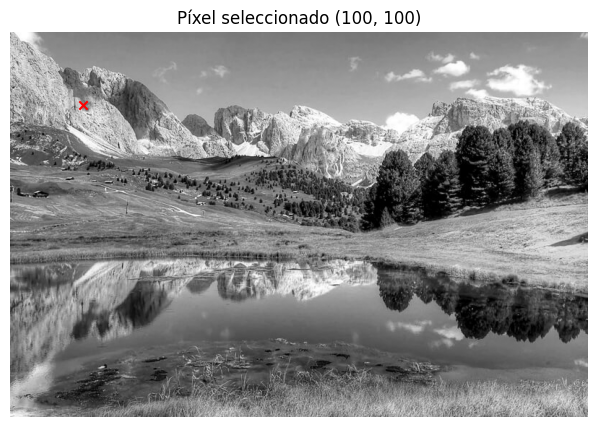
\includegraphics[width=0.75\textwidth]
    {../resultados/punto1.png}
    \caption{Píxel seleccionado en las coordenadas $(100,100)$.}
    \label{fig:punto1}
\end{figure}

La prueba permitió verificar que el origen de coordenadas se encuentra en la esquina superior izquierda de la imagen.

La coordenada $x$ aumenta hacia la derecha y la coordenada $y$ aumenta hacia abajo.


% =========================================================
\subsection{Punto 3: Aplicación sobre PIANO.bmp}

El algoritmo fue probado con las cinco coordenadas solicitadas.

Para:

\[
(82,29)
\]

se obtuvo:

\[
\begin{bmatrix}
53 & 65 & 103\\
50 & -1 & 105\\
50 & 68 & 116
\end{bmatrix}
\]

con píxel central de intensidad 63.

Para:

\[
(68,27)
\]

se obtuvo:

\[
\begin{bmatrix}
62 & 62 & 61\\
62 & -1 & 59\\
61 & 64 & 58
\end{bmatrix}
\]

con píxel central de intensidad 63.

Para:

\[
(112,89)
\]

se obtuvo:

\[
\begin{bmatrix}
66 & 61 & 64\\
66 & -1 & 63\\
62 & 58 & 63
\end{bmatrix}
\]

con píxel central de intensidad 59.

Para:

\[
(114,89)
\]

se obtuvo:

\[
\begin{bmatrix}
64 & 91 & 103\\
63 & -1 & 106\\
63 & 73 & 93
\end{bmatrix}
\]

con píxel central de intensidad 86.

Finalmente, para:

\[
(27,130)
\]

se obtuvo:

\[
\begin{bmatrix}
90 & 102 & 90\\
97 & -1 & 82\\
102 & 87 & 81
\end{bmatrix}
\]

con intensidad central 93.

Los resultados muestran diferencias entre regiones.

Por ejemplo, en $(68,27)$ los valores se encuentran aproximadamente entre 58 y 64, lo cual indica una zona relativamente homogénea.

En cambio, alrededor de $(82,29)$ aparecen intensidades entre aproximadamente 50 y 116, lo que representa una variación local mayor.

Esto demuestra que la vecindad puede utilizarse para analizar la estructura local de una imagen.


% =========================================================
\subsection{Punto 4: Ecualización local}

Para este punto se utilizó la imagen \texttt{PIANO.pgm}.

La media local se calculó mediante:

\begin{lstlisting}
media_local = cv2.blur(
    imagen_float,
    (3,3)
)
\end{lstlisting}

La función \texttt{cv2.blur()} calcula el promedio de una ventana que se desplaza sobre toda la imagen.

Para obtener la desviación estándar se utilizó:

\[
\sigma^2
=
E[x^2]-E[x]^2
\]

implementado mediante:

\begin{lstlisting}
media_cuadrados = cv2.blur(
    imagen_float**2,
    (3,3)
)

varianza_local = (
    media_cuadrados
    - media_local**2
)

desviacion_estandar_local = np.sqrt(
    np.maximum(varianza_local, 0)
)
\end{lstlisting}

Posteriormente se calculó el factor:

\begin{lstlisting}
A = (
    k * media_global
    / (desviacion_estandar_local + epsilon)
)
\end{lstlisting}

y la imagen transformada:

\begin{lstlisting}
imagen_local = (
    A * (imagen_float - media_local)
    + media_local
)

imagen_local = np.clip(
    imagen_local,
    0,
    255
).astype(np.uint8)
\end{lstlisting}

El resultado se observa en la
\hyperref[fig:ecualizacion-local]{Figura~\ref*{fig:ecualizacion-local}}.

\begin{figure}[H]
    \centering
    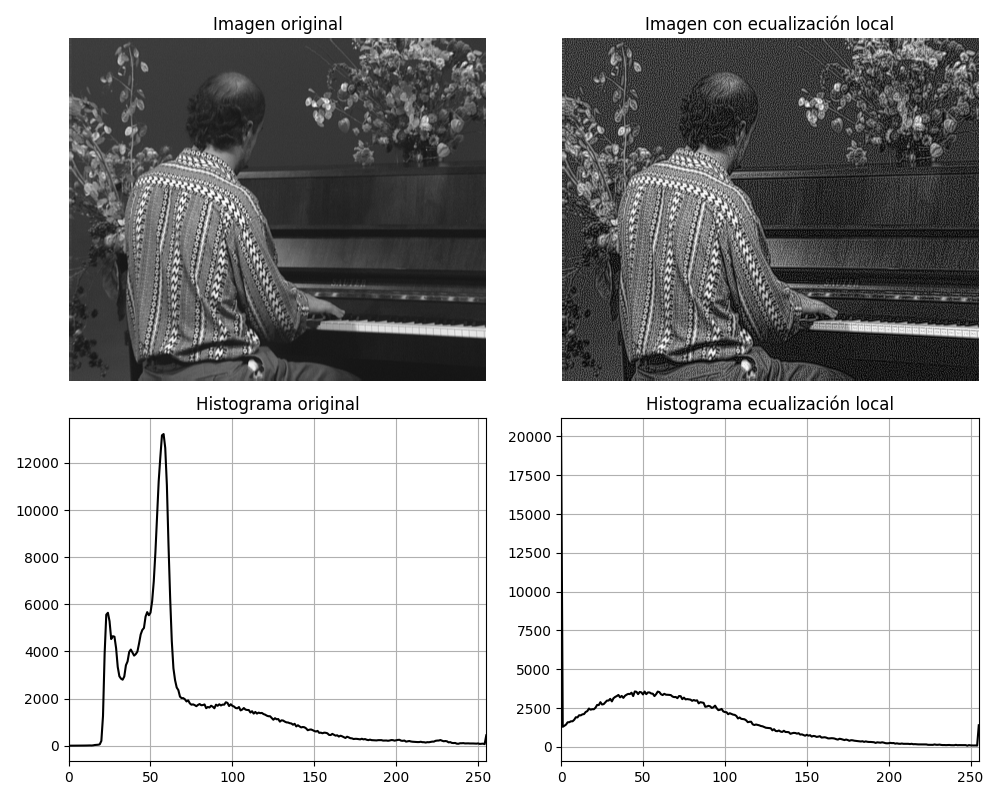
\includegraphics[width=\textwidth]
    {../resultados/ecualizacion_local_pt4.png}
    \caption{Imagen original, ecualización local y comparación de histogramas.}
    \label{fig:ecualizacion-local}
\end{figure}

En la imagen transformada se observa un aumento fuerte del contraste local, especialmente en texturas del cabello, ropa, piano y plantas.

El histograma también cambia considerablemente.

Un resultado importante fue la concentración de aproximadamente 20153 píxeles en intensidad 0. Esto ocurre porque algunos valores transformados quedan por debajo de cero y posteriormente son limitados mediante:

\begin{lstlisting}
np.clip(valor, 0, 255)
\end{lstlisting}

La técnica realza detalles, pero puede producir una modificación excesiva cuando la desviación estándar local es muy pequeña.


% =========================================================
\subsection{Punto 5: Ecualización local manual mediante ciclos}

En este punto se implementó el mismo procedimiento utilizando ciclos.

Para cada píxel se tomó una ventana de $3\times3$:

\begin{lstlisting}
ventana = imagen_float[
    fila-1:fila+2,
    columna-1:columna+2
]
\end{lstlisting}

Posteriormente se calcularon:

\begin{lstlisting}
media_local = np.mean(ventana)

desviacion_estandar_local = (
    np.std(ventana)
)
\end{lstlisting}

El factor de realce se calculó mediante:

\begin{lstlisting}
if desviacion_estandar_local != 0:
    A = (
        k * media_global
        / desviacion_estandar_local
    )
else:
    A = Amax
\end{lstlisting}

A diferencia del punto anterior, el factor fue limitado mediante:

\begin{equation}
0.5 \leq A(i,j) \leq 2.5
\end{equation}

utilizando:

\begin{lstlisting}
A = np.clip(A, Amin, Amax)
\end{lstlisting}

La transformación del píxel central fue:

\begin{lstlisting}
pixel_transformado = (
    A * (pixel_original - media_local)
    + media_local
)
\end{lstlisting}

El resultado se muestra en la
\hyperref[fig:ecualizacion-manual]{Figura~\ref*{fig:ecualizacion-manual}}.

\begin{figure}[H]
    \centering
    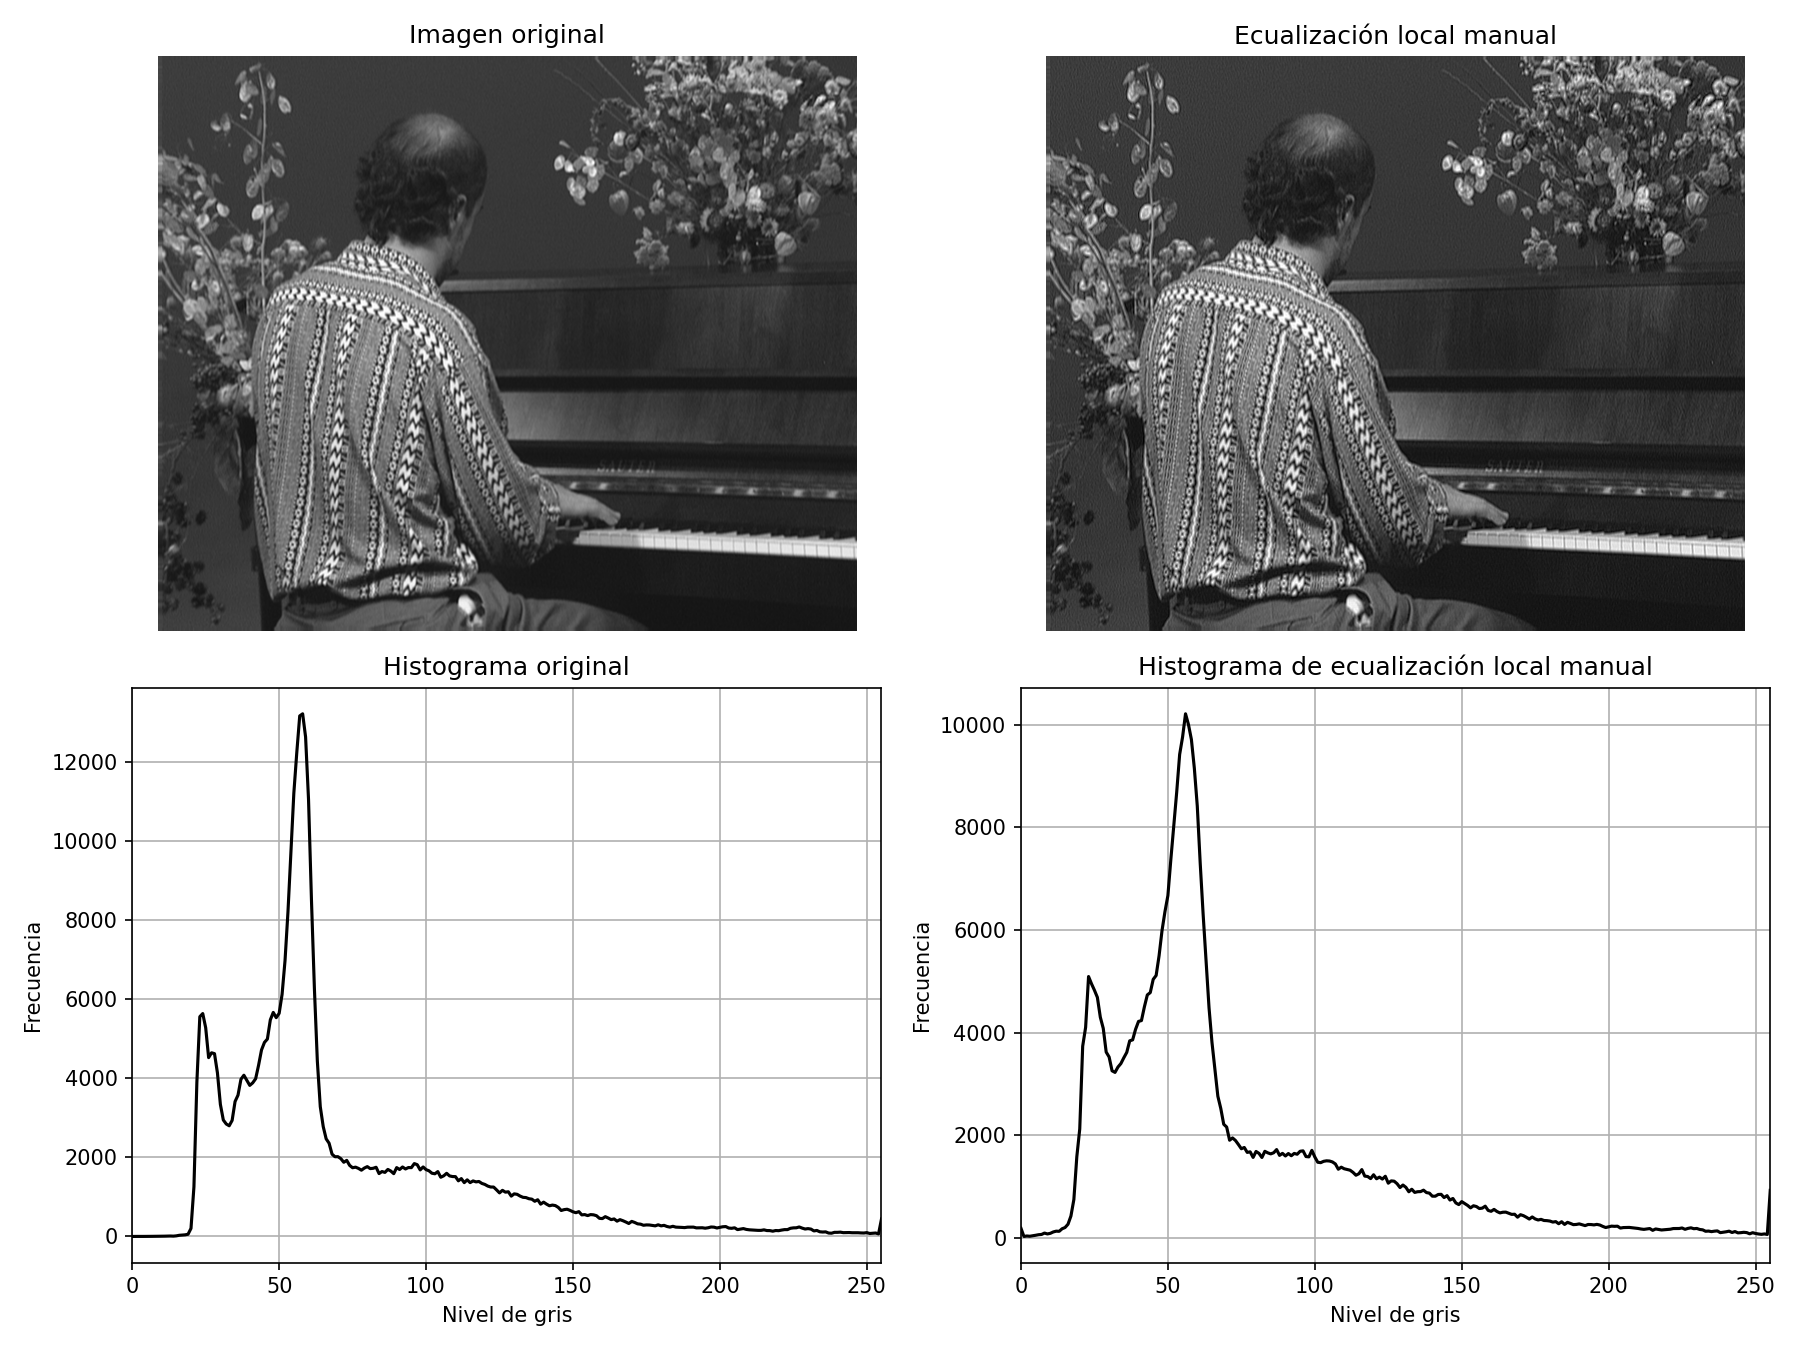
\includegraphics[width=\textwidth]
    {../resultados/ecualizacion_local_manual_pt5.png}
    \caption{Ecualización local implementada mediante ciclos y comparación de histogramas.}
    \label{fig:ecualizacion-manual}
\end{figure}

Los valores obtenidos fueron:

\begin{itemize}
    \item Promedio original: 72.14.
    \item Promedio transformado: 71.69.
    \item Intensidad mínima original: 1.
    \item Intensidad máxima original: 255.
    \item Intensidad mínima transformada: 0.
    \item Intensidad máxima transformada: 255.
    \item Total de píxeles: 403200.
\end{itemize}

La imagen transformada conserva una apariencia mucho más parecida a la original que la obtenida en el punto 4.

Esto se debe a que el factor $A$ está limitado.

Mientras en el punto anterior más de 20000 píxeles llegaron al valor 0, en esta implementación solamente 185 píxeles terminaron en dicha intensidad.

Por lo tanto, limitar $A$ evita un realce excesivo y permite mejorar el contraste local de manera más estable.


% =========================================================
\subsection{Punto 6: Operaciones lógicas entre imágenes}

Primero se cargaron y binarizaron las imágenes:

\begin{lstlisting}
bin_grande = cv2.threshold(
    imagen_grande,
    127,
    255,
    cv2.THRESH_BINARY
)[1]

bin_chica = cv2.threshold(
    imagen_chica,
    127,
    255,
    cv2.THRESH_BINARY
)[1]
\end{lstlisting}

Luego se creó una función basada en ciclos:

\begin{lstlisting}
def operacion_logica(
    imagen_a,
    imagen_b,
    operacion
):

    filas, columnas = imagen_a.shape

    resultado = np.zeros(
        (filas, columnas),
        dtype=np.uint8
    )

    for fila in range(filas):
        for columna in range(columnas):

            pixel1 = imagen_a[
                fila,
                columna
            ]

            pixel2 = imagen_b[
                fila,
                columna
            ]

            if operacion == "AND":
                resultado[fila, columna] = (
                    pixel1 & pixel2
                )

            elif operacion == "OR":
                resultado[fila, columna] = (
                    pixel1 | pixel2
                )

            elif operacion == "XOR":
                resultado[fila, columna] = (
                    pixel1 ^ pixel2
                )

    return resultado
\end{lstlisting}

Para NOT se desarrolló una función independiente:

\begin{lstlisting}
def operacion_not(imagen):

    filas, columnas = imagen.shape

    resultado = np.zeros(
        (filas, columnas),
        dtype=np.uint8
    )

    for fila in range(filas):
        for columna in range(columnas):

            if imagen[fila, columna] == 0:
                resultado[fila, columna] = 255
            else:
                resultado[fila, columna] = 0

    return resultado
\end{lstlisting}

Los resultados se muestran en la
\hyperref[fig:operaciones-logicas]{Figura~\ref*{fig:operaciones-logicas}}.

\begin{figure}[H]
    \centering
    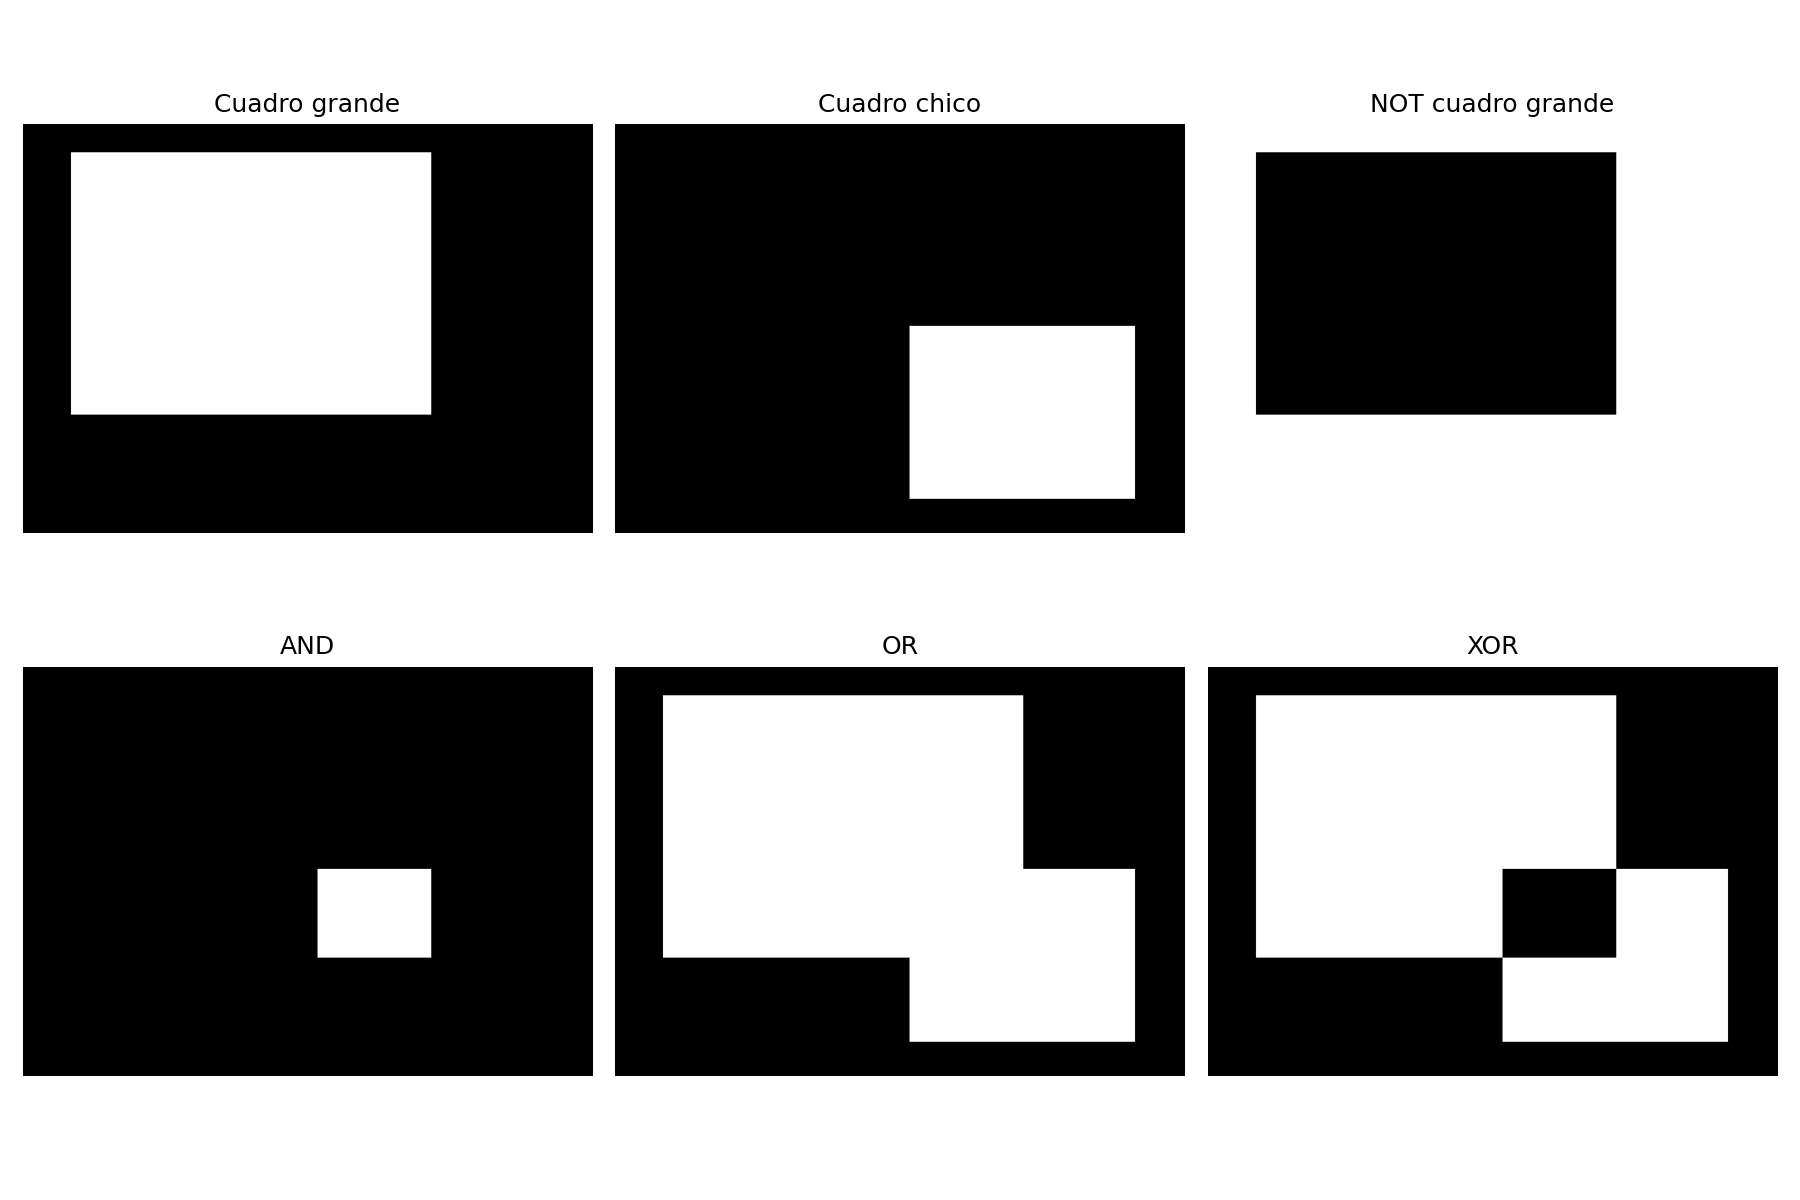
\includegraphics[width=\textwidth]
    {../resultados/operaciones_logicas_pt6.png}
    \caption{Resultados de las operaciones NOT, AND, OR y XOR.}
    \label{fig:operaciones-logicas}
\end{figure}

El resultado de AND corresponde únicamente a la región donde ambos cuadros blancos coinciden.

OR representa la unión de las regiones blancas.

XOR conserva las zonas donde las dos imágenes son diferentes, eliminando la intersección.

Finalmente, NOT invierte los valores de la imagen binaria.


% =========================================================
\section{Análisis general}

El taller permitió observar que muchas técnicas de procesamiento digital de imágenes dependen de la información espacial existente alrededor de cada píxel.

En los primeros ejercicios se comprobó que una vecindad permite conocer si una región es homogénea o si presenta cambios importantes de intensidad.

La ecualización local mostró que estas propiedades pueden utilizarse para modificar el contraste de manera diferente en cada zona de una imagen.

Cuando la desviación estándar local es pequeña, el factor de realce puede aumentar considerablemente. Por esta razón, si no se limita el valor de $A$, pueden aparecer saturaciones en 0 y 255.

La comparación entre los puntos 4 y 5 evidenció que limitar:

\[
0.5 \leq A(i,j) \leq 2.5
\]

permite obtener una transformación más controlada.

Finalmente, las operaciones lógicas permitieron trabajar con imágenes binarias como conjuntos de regiones. AND permitió obtener intersecciones, OR uniones, XOR diferencias y NOT el complemento de una imagen.


% =========================================================
\section{Conclusiones}

La vecindad de ocho píxeles constituye una herramienta fundamental para estudiar características locales de una imagen. La implementación realizada permitió obtener correctamente las intensidades que rodean un píxel seleccionado.

El análisis de diferentes coordenadas mostró que regiones con valores muy similares pueden considerarse homogéneas, mientras que una mayor variación entre vecinos puede indicar bordes, cambios de región o presencia de textura.

La ecualización local permitió comprobar que la media y la desviación estándar de una vecindad pueden utilizarse para modificar el contraste de manera adaptativa. La transformación no actúa igual sobre toda la imagen, sino que depende de las características de cada región.

También se observó que un factor de realce sin límites puede producir cambios excesivos y saturación. Limitar $A$ entre 0.5 y 2.5 permitió conservar mejor la apariencia original y mejorar el detalle local de forma más estable.

Las operaciones lógicas AND, OR, XOR y NOT funcionaron de acuerdo con sus tablas de verdad y demostraron su utilidad para combinar, separar e invertir regiones binarias.

En conjunto, el taller permitió comprender la relación entre \textbf{vecindad, estadísticas locales, contraste y operaciones lógicas}, conceptos fundamentales para técnicas posteriores como filtrado, detección de bordes, segmentación y reconocimiento de objetos.

\end{document}